\documentclass[10pt,UTF8]{ctexart}


\usepackage[margin=2cm,a4paper]{geometry}
%\usepackage[left=0.75in,top=0.6in,right=0.75in,bottom=1.0in,a4paper]{geometry}

\setmainfont{Caladea}
%% 也可以選用其它字庫:
% \setCJKmainfont[%
%   ItalicFont=AR PL KaitiM GB,
%   BoldFont=Noto Sans CJK SC,
% ]{Noto Serif CJK SC}
% \setCJKsansfont{Noto Sans CJK SC}
% \renewcommand{\kaishu}{\CJKfontspec{AR PL KaitiM GB}}

% 繁體中文
\setCJKmainfont[Path=fonts/ ]{NotoSansTC-Medium.otf}

\usepackage{minted}
\usepackage[breaklinks]{hyperref}

% Picture
% 導言區的此三行無變化
\usepackage{graphicx}
\usepackage{float} 
\usepackage{subfigure}
% 以下是新增的自定義格式更改
\usepackage[]{caption2} %新增調用的宏包
\renewcommand{\figurename}{Fig.} %重定義編號前綴詞
\renewcommand{\captionlabeldelim}{.~} %重定義分隔符
 %\roman 是羅馬數字編號,\alph是默認的字母編號,\arabic是阿拉伯數字編號,可按需替換下一行的相應位置
\renewcommand{\thesubfigure}{(\roman{subfigure})}%此外,還可設置圖編號顯示格式,加括號或者不加括號
\makeatletter \renewcommand{\@thesubfigure}{\thesubfigure \space}%子圖編號與名稱的間隔設置
\renewcommand{\p@subfigure}{} \makeatother

% Math
\usepackage {mathtools}
\usepackage{amssymb}

% Code
\usepackage{listings}
\usepackage{xcolor}
\lstset{
    % backgroundcolor=\color{red!50!green!50!blue!50},
    % 程式碼塊背景色為淺灰色
    rulesepcolor= \color{gray}, % 程式碼塊邊框顏色
    breaklines=true,  % 程式碼過長則換行
    numbers=left, % 行號在左側顯示
    numberstyle= \small,% 行號字型
    % eywordstyle= \color{red,% 關鍵字顏色
    commentstyle=\color{gray}, % 註釋顏色
    frame=shadowbox % 用方框框住程式碼塊
    }

\usepackage{hyperref}

\title{計算機視覺作業}
\author{干皓丞,2101212850, 信息工程學院}

\begin{document}
\maketitle


\section{作業目標與章節摘要}

1. 尋找一篇 2020/2021 年風格遷移的文章

2. 翻譯其摘要和貢獻;對程式碼主體部分進行註釋,截圖

3. 配置環境,測試自己的圖片進行風格遷移的結果,截圖

\section{文章與作業狀況}

作業可以從 GitHub 下的 kancheng/kan-cs-report-in-2021 專案找到,作業程式碼目錄為 kan-cs-report-in-2021/CV/style-transfer/code。實際執行的環境與實驗設備為 Google 的 Colab 、MacBook Pro (Retina, 15-inch, Mid 2014) 、 Acer Aspire R7 與 HP Victus (Nvidia GeForce RTX 3060)

Sunnie S. Y. Kim, Nicholas Kolkin, Jason Salavon, Gregory Shakhnarovich, 2020, Deformable Style Transfer, (ECCV 2020).

\section{摘要和貢獻}

在此將 ECCV 2020 的可變形風格轉移 (Deformable Style Transfer) 進行說明與整理。

原文摘要如下 :

Sunnie S. Y. Kim, Nicholas Kolkin, Jason Salavon, Gregory Shakhnarovich ;
Both geometry and texture are fundamental aspects of visual style. Existing style transfer methods, however, primarily focus on texture, almost entirely ignoring geometry. We propose deformable style transfer (DST), an optimization-based approach that jointly stylizes the texture and geometry of a content image to better match a style image. Unlike previous geometry-aware stylization methods, our approach is neither restricted to a particular domain (such as human faces), nor does it require training sets of matching style/content pairs. 
We demonstrate our method on a diverse set of content and style images including portraits, animals, objects, scenes, and paintings. Code has been made publicly available at https://github.com/sunniesuhyoung/DST."

原文摘要的中文整理如下:

幾何和紋理都是視覺風格的基本基礎,然而當下的的風格轉移方法都關注在紋理上,幾乎忽略幾何的部分,而研究者們提出提出了可變形樣式轉移 (DST; Deformable Style Transfer),此優化方法可聯合對內容圖像中的紋理和幾何形狀來進行樣式化,從而可以更好地匹配影像風格。於過往的幾何感知風格化方法不同,該研究的方法既不限於特定領域(例如人臉),也不需匹配樣式/內容到對的訓練資料集上。而研究者在一系列不同的內容和風格圖像上展示了我們的方法,包括肖像、動物、物體、場景和繪畫。


而該研究原文的前言與研究者們貢獻的中文簡略整理三段包含貢獻與部分原文對應如下:

研究者提出一個擴展風格遷移的方法,使之可更好地對應藝術家風格作品的幾何形狀上,而在過往樣式定義中並無明確包含幾何的樣式,其幾何的部份通過轉移方法後,再最後輸出的內容中是不變的。從而導致這些演算法的輸出會很容易被識別為內容圖像的更改或者是 "過濾" 版本,而非使用根據內容圖像作為參考,而創建的新圖像。而該篇研究的研究者們在這項工作中的專注部分為,於將形狀和幾何圖形去作為風格的重要標誌,並相互結合,同時放鬆對其內容的限制,使之作為一個可接收的 "畫布"。

該研究通過引入內容圖像的域不可知幾何變形來實現這一點,並與標準樣式轉移損失聯合優化(by introducing a domain-agnostic geometric deformation of the content image, optimized jointly with standard style transfer losses.)。而該研究提出的方法,可變形風格轉移 (DST;Deformable Style Transfer),則是將做為內容圖像和風格圖像(a content image and a style image)的兩張圖像進行輸入。研究者假設這兩個圖像共享一個域並且有一些近似對齊,所謂的近似對齊類於都是坐著的動物的圖像,這在用於娛樂或藝術用途以及數據增強等風格轉移的工作中很普遍。而此問題會使學習遷移風格變得具有挑戰性,因為無法合理地假設在任何可行的訓練集中捕捉到不受約束的領域和風格的變化。

而跟其他風格遷移工作類似,研究者們基於此開發了一種優化的方法,利用 ImageNet 分類訓練的卷積網絡 (CNN) 做預訓練和固定特徵提取。在此研究者也將關於學習幾何風格的工作,使用地標星座的顯式模型或代表特定風格的變形模型等需要一組所選風格的圖像,並且僅適用於特定領域的方法與自己的結果進行比較,發現我們的方法產生了同樣美觀的結果,儘管更為通用。

此工作中,研究提出了第一個,據研究者所知,將幾何融入一次性、領域不可知風格轉移的方法,其 DST 的關鍵思想是找到內容圖像的平滑變形或空間扭曲部分,使其與樣式圖像在空間上對齊。這種變形會由一組匹配的關鍵點引導,選擇最大化在兩幅圖像配對關鍵點間的特徵相似性。

該研究貢獻如下

– 提出一個優化框架,此框架賦予風格遷移算法顯式的能力,能夠使內容圖像變形以匹配風格圖像的幾何形狀。而且可以讓使用者利用公式來進行權衡化的風格控制。

– 首次在 oneshot 場景中展示了幾何感知風格轉移。與之前僅限於人臉的工作相比,DST 適用於其他領域的圖像,假設它們共享一個域並具有一些近似對齊。

– 我們在一系列風格轉移實例上評估 DST,包括面部、動物、車輛和風景的圖像,並通過使用者研究證明我們的框架可以增強現有的風格轉移算法,用最低的成本來顯著提高感知內容。

To summarize the contributions of this work:

– We propose an optimization-based framework that endows style transfer algorithms with the explicit ability to deform a content image to match the geometry of a style image. Our flexible formulation also allows explicit user guidance and control of stylization tradeoffs.

– We demonstrate, for the first time, geometry-aware style transfer in a oneshot scenario.
In contrast to previous works that are limited to human faces, DST works for images in other domains, with the assumption that they share a domain and have some approximate alignment.

– We evaluate DST on a range of style transfer instances, with images of faces, animals, vehicles, and landscapes, and through a user study demonstrate that our framework can augment existing style transfer algorithms to dramatically improve the perceived stylization quality, at minimal cost to the percieved content preservation.

\newpage

\section{原圖像測試與實驗結果對照}

其研究得專案內容程式碼為 sunniesuhyoung/DST,而自己實際測試該專案的範例程式碼在 code 目錄下的 demo\_DST\_Kan.ipynb 檔案。該檔案為 sunniesuhyoung/DST 專案下的專案範例說明 demo\_DST.ipynb。同時為了方便測試,此作業對原專案進行 Fork(kancheng/DST),對其在 Colab 進行測試。研究者範例使用兔子作為訓練範例,而這裡則使用 Google 隨機抓來的無尾熊兩張圖片進行測試,看最後呈現的結果。 

\begin{figure}[H]
\centering 
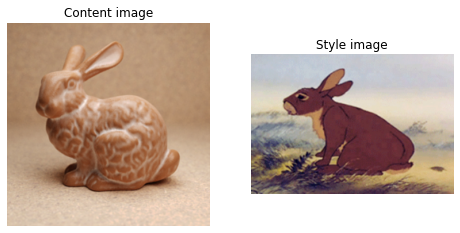
\includegraphics[width=0.50\textwidth]{r1.png} 
\caption{原研究者兔子版本}
\label{Test}
\end{figure}

\begin{figure}[H]
\centering 
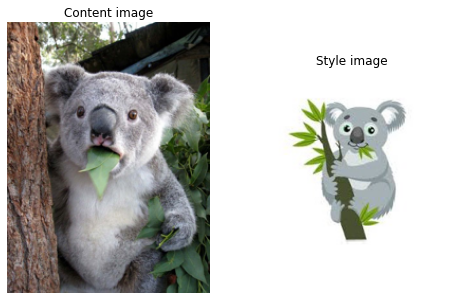
\includegraphics[width=0.50\textwidth]{t1.png} 
\caption{實驗無尾熊版本}
\label{Test}
\end{figure}

在此進行幾何圖形的定位點測試,可以看到照片版本的無尾熊和卡通圖像的無尾熊的點,其大多數都定位到相應位置。

\begin{figure}[H]
\centering 
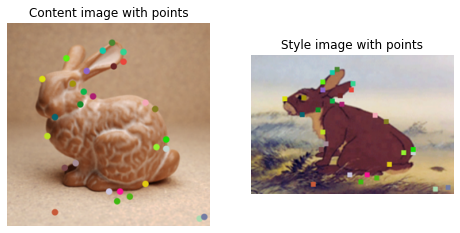
\includegraphics[width=0.50\textwidth]{r2.png} 
\caption{原研究者兔子的定位點版本}
\label{Test}
\end{figure}

\begin{figure}[H]
\centering 
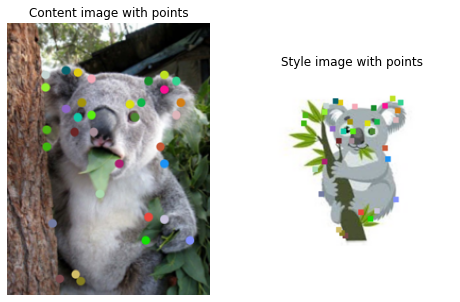
\includegraphics[width=0.50\textwidth]{t2.png} 
\caption{實驗無尾熊的定位點版本}
\label{Test}
\end{figure}

而最後訓練完後則可以看到一個有趣的結果,最後產生的風格類似於卡通,而無尾熊的抱的樹則被換成了灰色。而原研究者的兔子也是有類似特色,產生出來的兔子有著卡通版本的兔子相近的色調。

\begin{figure}[H]
\centering 
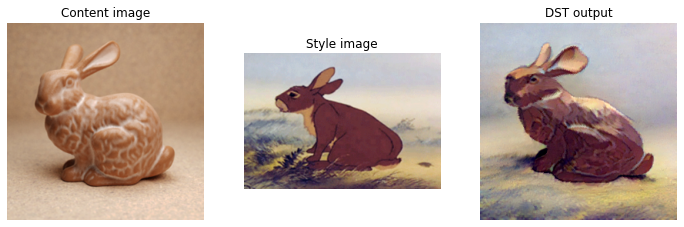
\includegraphics[width=0.50\textwidth]{r3.png} 
\caption{DST 兔子}
\label{Test}
\end{figure}

\begin{figure}[H]
\centering 
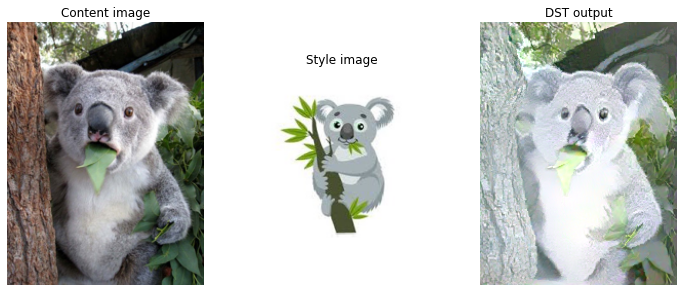
\includegraphics[width=0.80\textwidth]{t3.png} 
\caption{DST 無尾熊}
\label{Test}
\end{figure}

\newpage

\section{測試環境配置過程紀錄與說明}

Google 的 Colab 可以將預先要測試的 Code 與專案運用 GitHub 與 Git 指令 (git clone),將整個測試專案提交到預定的 GitHub 上,並用指令操作目錄執行預定地 Python 檔案,從而簡單明瞭的進行測試與呈現結果。實際測試需要 CUDA 與 GPU 穩定的實驗環境才可以。

\begin{figure}[H]
\centering 
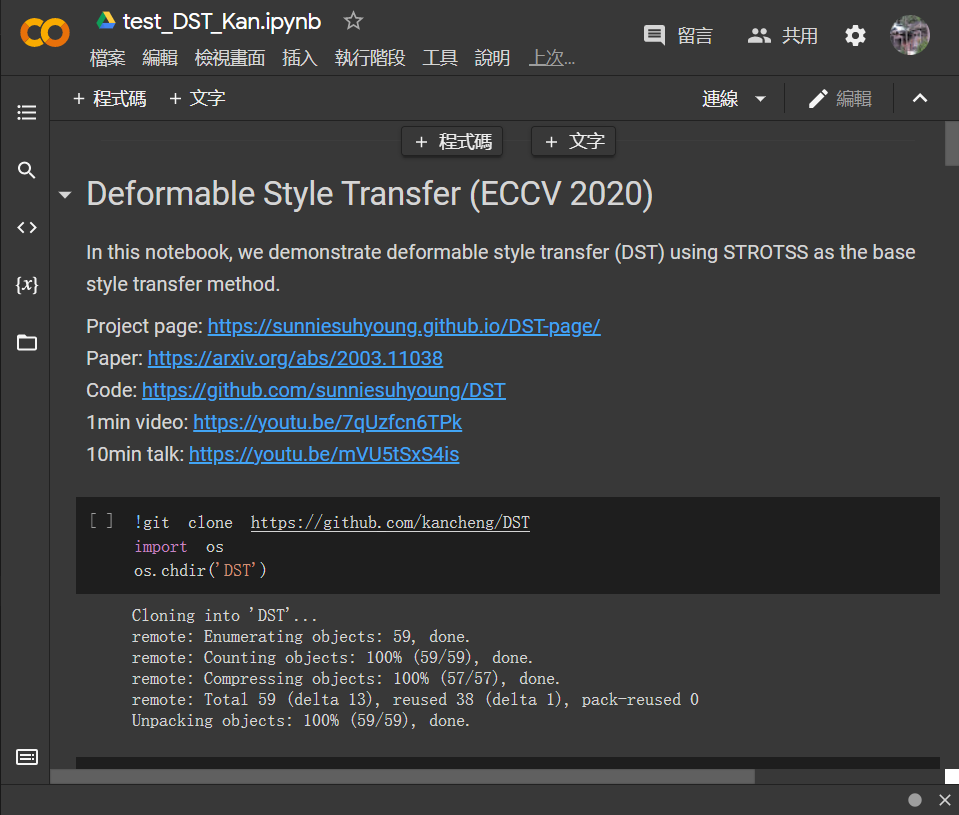
\includegraphics[width=0.80\textwidth]{c1.png} 
\caption{Colab 修改後的研究測試範例}
\label{Test}
\end{figure}

\begin{figure}[H]
\centering 
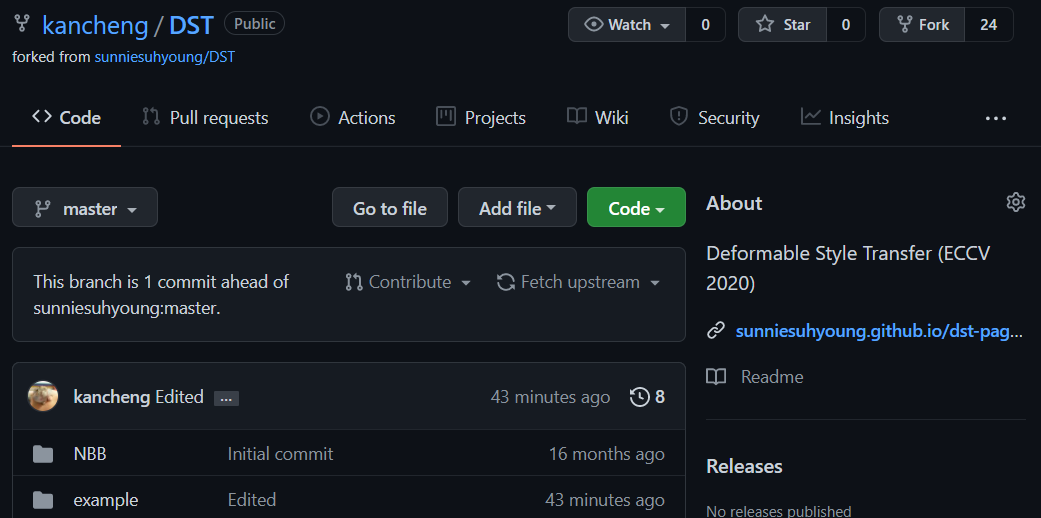
\includegraphics[width=0.80\textwidth]{c2.png} 
\caption{GitHub - Fork 過後的且修改測試的專案}
\label{Test}
\end{figure}

\newpage

\section{整體專案與程式碼說明}

在此專案除了兩個名為 demo\_DST.ipynb 和 demo\_warp.ipynb 的測試專案範例程式碼之外,整體由 main.py 執行,main,py 執行時會叫 vggfeatures.py 也就是 VGG 和 styletransfer.py 的 DST,而 styletransfer.py 在此會叫到其他支援的 Python 檔案。

\begin{figure}[H]
\centering 
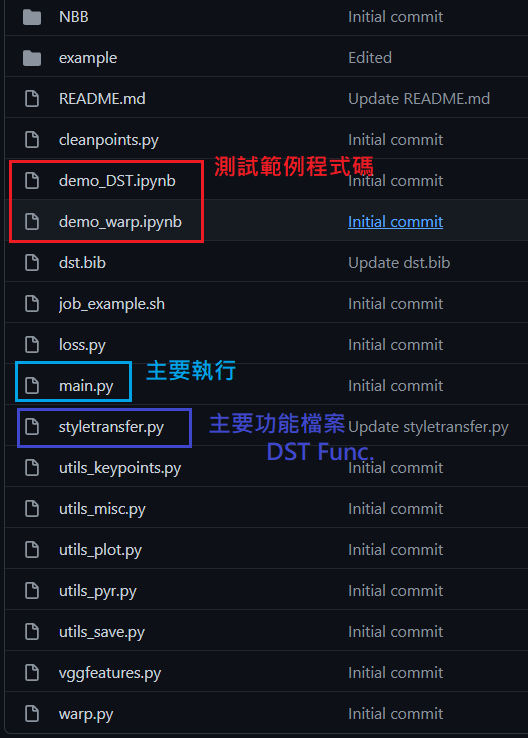
\includegraphics[width=0.30\textwidth]{p1.png} 
\caption{整體專案目錄}
\label{Test}
\end{figure}

\begin{figure}[H]
\centering 
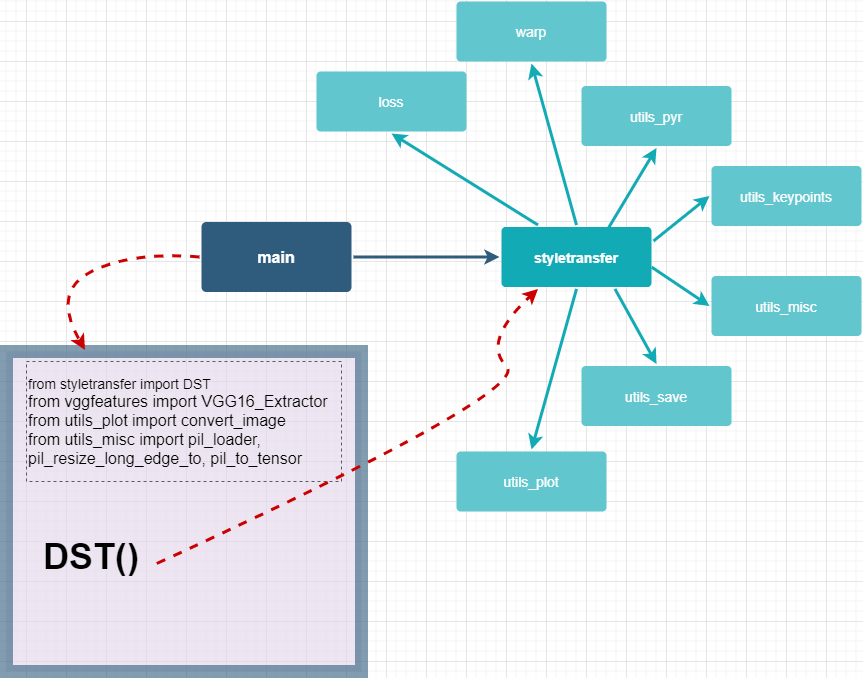
\includegraphics[width=0.80\textwidth]{p2.png} 
\caption{整體專案架構}
\label{Test}
\end{figure}

\newpage

由上圖得知,styletransfer.py 為整個 DST 最重要的 Python 檔案,以下用程式碼配合中文註解的方式進行說明。

\begin{lstlisting}[language={python}]
# 在此匯入基本的 Python 套件。
import time
import numpy as np
import matplotlib.pyplot as plt
import torch
import torch.nn.functional as F
from torch.autograd import Variable

# 匯入專案的各部分 Python 檔案與功能,包含繪圖、損失、點、圖片處理等。
from loss import content_loss, remd_loss, moment_loss, TV, pairwise_distances_sq_l2
from warp import apply_warp
from utils_pyr import syn_lap_pyr, dec_lap_pyr
from utils_keypoints import init_keypoint_params, gen_dst_pts_keypoints
from utils_misc import sample_indices, spatial_feature_extract
from utils_save import save_loss, save_points
from utils_plot import save_plots, plot_intermediate

# DST 函數定義,可以看到各個參數,輸入、風格、內容、風格檔案路徑、內容檔案路徑
# 包含 checkpoint、是否用到 GPU。
def DST(input_im, content_im, style_im, extractor, content_path, style_path,
        content_pts, style_pts, style_pts_path, output_dir, output_prefix,
        im_size = 256,
        max_iter = 250,
        checkpoint_iter = 50,
        content_weight = 8.,
        warp_weight = 0.3,
        reg_weight = 10,
        scales = 3,
        pyr_levs = 5,
        sharp_warp = False,
        optim = 'adam',
        lr = 1e-3,
        warp_lr_fac = 1.,
        verbose = False,
        save_intermediate = False,
        save_extra = False,
        device = 'cuda:0'):
    # 如果 warp weight 權重為 0,則運行基本方法為 STROTSS
    # If warp weight is 0, run the base method STROTSS
    use_DST = True
    if warp_weight == 0.:
        use_DST = False
    # 初始化 warp 參數。
    # Initialize warp parameters
    src_Kpts, target_Kpts, border_Kpts, no_flow_Kpts= init_keypoint_params(input_im, content_path, content_pts, style_pts, device)
    thetas_Kpts = Variable(torch.rand_like(src_Kpts).data*1e-4, requires_grad=True)
    # 夾住目標點,使之不會超過邊界
    # Clamp the target points so that they don't go outside the boundary
    target_Kpts[:,0] = torch.clamp(target_Kpts[:,0], min=5, max=content_im.size(2)-5)
    target_Kpts[:,1] = torch.clamp(target_Kpts[:,1], min=5, max=content_im.size(3)-5)
    target_Kpts_o = target_Kpts.clone().detach()
    # 為每組點分配不同的顏色,方便使用者用於視覺化的觀察。
    # Assign colors to each set of points (used for visualization only)
    np.random.seed(1)
    colors = []
    for j in range(src_Kpts.shape[0]):
        colors.append(np.random.random(size=3))
    # 初始化 pixel 參數
    # Initialize pixel parameters
    s_pyr = dec_lap_pyr(input_im, pyr_levs)
    s_pyr = [Variable(li.data, requires_grad=True) for li in s_pyr]
    
    # 定義 參數給 optimized
    # Define parameters to be optimized
    s_pyr_list = [{'params': si} for si in s_pyr]
    if use_DST:
        thetas_opt_list = [{'params': thetas_Kpts, 'lr': lr*warp_lr_fac}]
    else:
        thetas_opt_list = []
    # 構造 優化器(optimizer)
    # Construct optimizer
    if optim == 'sgd':
        optimizer = torch.optim.SGD(s_pyr_list + thetas_opt_list, lr=lr, momentum=0.9)
    elif optim == 'rmsprop':
        optimizer = torch.optim.RMSprop(s_pyr_list + thetas_opt_list, lr=lr)
    else:
        optimizer = torch.optim.Adam(s_pyr_list + thetas_opt_list, lr=lr)
    # 設定 scales
    # Set scales
    scale_list = list(range(scales))
    if scales == 1:
        scale_list = [0]
    # 建立 lists 的空資料給 store various loss values
    # Create lists to store various loss values
    ell_list = []
    ell_style_list = []
    ell_content_list = []
    ell_warp_list = []
    ell_warp_TV_list = []

    # 在圖像上迭代其風格
    # Iteratively stylize over more levels of image pyramid
    for scale in scale_list:

        down_fac = 2**(scales-1-scale)
        begin_ind = (scales-1-scale)
        content_weight_scaled = content_weight*down_fac

        print('\nOptimizing at scale {}, image size ({}, {})'.format(scale+1, content_im.size(2)//down_fac, content_im.size(3)//down_fac))

        if down_fac > 1.:
            content_im_scaled = F.interpolate(content_im, (content_im.size(2)//down_fac, content_im.size(3)//down_fac), mode='bilinear')
            style_im_scaled = F.interpolate(style_im, (style_im.size(2)//down_fac, style_im.size(3)//down_fac), mode='bilinear')
        else:
            content_im_scaled = content_im.clone()
            style_im_scaled = style_im.clone()
        # 計算在這個比例下不會改變的特徵圖
        # Compute feature maps that won't change for this scale
        with torch.no_grad():
            feat_content = extractor(content_im_scaled)

            feat_style = None
            for i in range(5):
                with torch.no_grad():
                    feat_e = extractor.forward_samples_hypercolumn(style_im_scaled, samps=1000)
                    feat_style = feat_e if feat_style is None else torch.cat((feat_style, feat_e), dim=2)

            feat_max = 3 + 2*64 + 2*128 + 3*256 + 2*512 # 2179 = sum of all extracted channels
            spatial_style = feat_style.view(1, feat_max, -1, 1)

            xx, xy = sample_indices(feat_content[0], feat_style)

        # 開始優化此規模
        # Begin optimization for this scale
        for i in range(max_iter):

            optimizer.zero_grad()
            # 從 laplacian pyramid 獲取當前的風格化圖像
            # Get current stylized image from the laplacian pyramid
            curr_im = syn_lap_pyr(s_pyr[begin_ind:])
            new_im = curr_im.clone()
            content_im_warp = content_im_scaled.clone()
            
            # 使用當前的 thetas 生成目標點
            # Generate destination points with the current thetas
            src_Kpts_aug, dst_Kpts_aug, flow_Kpts_aug = gen_dst_pts_keypoints(src_Kpts, thetas_Kpts, no_flow_Kpts, border_Kpts)
            # 計算 warp loss
            # Calculate warp loss
            ell_warp = torch.norm(target_Kpts_o - dst_Kpts_aug[:target_Kpts.size(0)], dim=1).mean()

            # Scale points to [0-1]
            src_Kpts_aug = src_Kpts_aug/torch.max(src_Kpts_aug, 0, keepdim=True)[0]
            dst_Kpts_aug = dst_Kpts_aug/torch.max(dst_Kpts_aug, 0, keepdim=True)[0]
            dst_Kpts_aug = torch.clamp(dst_Kpts_aug, min=0., max=1.)

            # Warp
            new_im, content_im_warp, warp_field = apply_warp(new_im, [src_Kpts_aug], [dst_Kpts_aug], device, sharp=sharp_warp, im2=content_im_warp)
            new_im = new_im.to(device)

            # Calculate total variation
            ell_warp_TV = TV(warp_field)

            # Extract VGG features of warped and unwarped stylized images
            feat_result_warped = extractor(new_im)
            feat_result_unwarped = extractor(curr_im)

            # Sample features to calculate losses with
            n = 2048
            if i % 1 == 0 and i != 0:
                np.random.shuffle(xx)
                np.random.shuffle(xy)
            spatial_result_warped, spatial_content = spatial_feature_extract(feat_result_warped, feat_content, xx[:n], xy[:n])
            spatial_result_unwarped, _ = spatial_feature_extract(feat_result_unwarped, feat_content, xx[:n], xy[:n])

            # Content loss
            ell_content = content_loss(spatial_result_unwarped, spatial_content)

            # Style loss

            # Lstyle(Unwarped X, S)
            loss_remd1 = remd_loss(spatial_result_unwarped, spatial_style, cos_d=True)
            loss_moment1 = moment_loss(spatial_result_unwarped, spatial_style, moments=[1,2])
            loss_color1 = remd_loss(spatial_result_unwarped[:,:3,:,:], spatial_style[:,:3,:,:], cos_d=False)
            loss_style1 = loss_remd1 + loss_moment1 + (1./max(content_weight_scaled, 1.))*loss_color1

            # Lstyle(Warped X, S)
            loss_remd2 = remd_loss(spatial_result_warped, spatial_style, cos_d=True)
            loss_moment2 = moment_loss(spatial_result_warped, spatial_style, moments=[1,2])
            loss_color2 = remd_loss(spatial_result_warped[:,:3,:,:], spatial_style[:,:3,:,:], cos_d=False)
            loss_style2 = loss_remd2 + loss_moment2 + (1./max(content_weight_scaled, 1.))*loss_color2

            # Total loss
            if use_DST:
                ell_style = loss_style1 + loss_style2
                ell = content_weight_scaled*ell_content + ell_style + warp_weight*ell_warp + reg_weight*ell_warp_TV
            else:
                ell_style = loss_style1
                ell = content_weight_scaled*ell_content + ell_style

            # Record loss values
            ell_list.append(ell.item())
            ell_content_list.append(ell_content.item())
            ell_style_list.append(ell_style.item())
            ell_warp_list.append(ell_warp.item())
            ell_warp_TV_list.append(ell_warp_TV.item())

            # Output intermediate loss
            if i==0 or i%checkpoint_iter == 0:
                print('   STEP {:03d}: Loss {:04.3f}'.format(i, ell))
                if verbose:
                    print('             = alpha*Lcontent {:04.3f}'.format(content_weight_scaled*ell_content))
                    print('               + Lstyle {:04.3f}'.format(ell_style))
                    print('               + beta*Lwarp {:04.3f}'.format(warp_weight*ell_warp))
                    print('               + gamma*TV {:04.3f}'.format(reg_weight*ell_warp_TV))
                if save_intermediate:
                    plot_intermediate(new_im, content_im_warp, output_dir, output_prefix, colors,
                                        down_fac, src_Kpts, thetas_Kpts, target_Kpts, scale, i)

            # Take a gradient step
            ell.backward()
            optimizer.step()


    # Optimization finished
    src_Kpts_aug, dst_Kpts_aug, flow_Kpts_aug = gen_dst_pts_keypoints(src_Kpts, thetas_Kpts, no_flow_Kpts, border_Kpts)
    sizes = torch.FloatTensor([new_im.size(2), new_im.size(3)]).to(device)
    src_Kpts_aug = src_Kpts_aug/sizes
    dst_Kpts_aug = dst_Kpts_aug/sizes
    dst_Kpts_aug = torch.clamp(dst_Kpts_aug, min=0., max=1.)
    dst_Kpts = dst_Kpts_aug[:src_Kpts.size(0)]

    # Apply final warp
    sharp_final = True
    new_im = curr_im.clone()
    content_im_warp = content_im.clone()
    new_im, _ = apply_warp(new_im, [src_Kpts_aug], [dst_Kpts_aug], device, sharp=sharp_final)

    # Optionally save loss, keypoints, and optimized warp parameter thetas
    if save_extra:
        save_plots(im_size, curr_im, new_im, content_im, style_im, output_dir, output_prefix, style_path, style_pts_path, colors,
                    src_Kpts, src_Kpts_aug, dst_Kpts*sizes, dst_Kpts_aug, target_Kpts, target_Kpts_o, border_Kpts, device)
        save_loss(output_dir, output_prefix, content_weight, warp_weight, reg_weight, max_iter, scale_list,
                    ell_list, ell_style_list, ell_content_list, ell_warp_list, ell_warp_TV_list)
        save_points(output_dir, output_prefix, src_Kpts, dst_Kpts*sizes, src_Kpts_aug*sizes,
                    dst_Kpts_aug*sizes, target_Kpts, thetas_Kpts)

    # Return the stylized output image
    return new_im
\end{lstlisting}

\section{數學說明}

在此根據該研究團隊的數學意義說明影片,進行簡易的處理再製後配合文字說明如下圖所示,可以看到參數、輸入、輸出各部分的說明。

\begin{figure}[H]
\centering 
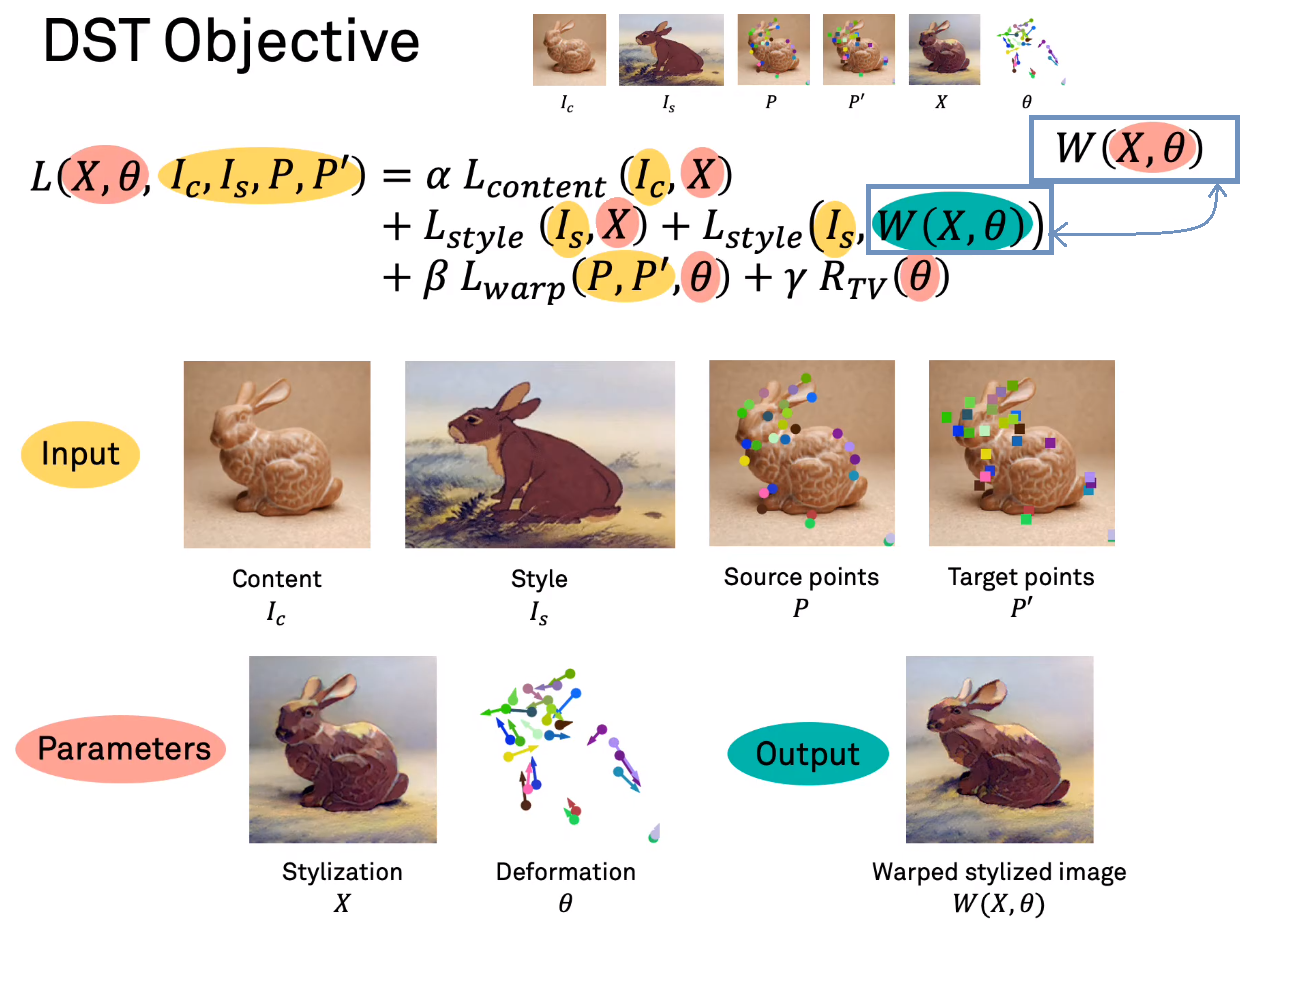
\includegraphics[width=0.80\textwidth]{m1.png} 
\caption{數學說明}
\label{Test}
\end{figure}

數學部分如下所示 :

$$L\left(X,\theta,I_c,I_s,P,P^\prime\right)=\alpha L_{content}\left(I_c,X\right)+L_{style}(I_s,X)+L_{style}(I_s,W(X,\theta))+\beta L_{warp}(P,P\prime,\theta)+\gamma R_{TV}(\theta)$$

1. $L_{content} (I_{c},X)$: Content loss of the base style transfer method.

基本風格遷移方法的內容損失。

2. $L_{style} (I_{s}, X)$: Style loss of the base style transfer method.

基礎風格遷移方法的風格損。

3. $L_{style} (I_{s}, W(X,\theta))$: Style loss applied to the warped stylized image.

應用於扭曲的風格化圖像的樣式損失。

4. $L_{warp}(P, P', \theta)$: Mean $l_{2}$ distance between optimized and target points.

優化點和目標點之間的平均$l_{2}$距離。

5. $R_{TV}(e)$: Total variation norm of the 2D warp field.

2D warp field 的總變化範數。

6. $ \alpha $ and $ \beta $ : $ \alpha $ and $ \beta $ are hyperparameters that control the relative importance of content preservation and deformation to stylization.

$ \alpha $ 和 $ \beta $ 是控制內容保存和變形對風格化的相對重要性的 hyperparameters。

7. $ \gamma $ : $ \gamma $ controls the amount of regularization on the deformation.

$ \gamma $ 控制變形的正則化量。

We use stand iterative optimization techniques such as stochastic gradient descent to minimize the subjective with respect to $X$ and $\theta$.

我們使用 stand iterative optimization techniques,例如隨機梯度下降來最小化關於 $X$ 和 $\theta$ 的 subjective。



% 數學意義說明

% $$\min \limits_{G}\max \limits_{D}{V_I(D,\ G)=V(D,G)-\lambda L_I(G,Q)}$$

%	\begin{lstlisting}[language={python}]

%	\end{lstlisting}

%\begin{enumerate}
%\item Y
%\item A
%\end{enumerate}

% \newpage

\clearpage

\end{document}